\chapter{Trusted computing}
Nowadays, the modern computing system is made up of many highly
distributed components.

Let's take into consideration the typical distributed infrastructure,
it's made up of a cloud for storage and computation, which communicate
with other devices outside its cluster, such as IoT devices, via edge
routers. Securing all those components it's a real challenge, because
each of those devices could be different, as well as their
communication technologies(Wired, Wireless, etc.). 

While in the past we had physical components, nowadays the trend is
\textbf{softwarization of the components} on top of a generic
commodity hardware, with "tools" such as SDN, NVF, etc.
\begin{boxH}
  As a consequence, systems \textbf{more flexible} but \textbf{more
  vulnerable}.
\end{boxH}
After all, the larger the software base, the higher the probability of
bugs, especially in the software, but hardware bugs are to be taken 
into consideration as well. All this without even considering the
issue of software updates

One of the main issues nowadays is \textbf{trustworthiness}, that being if
something behaves exactly as expected. However, there are several problems
related to trust in this context:

\begin{itemize}
    \item Trust in the cloud provider(s)
    \item Trust in the network/edge provider(s)
    \item Low or no access control for edge- and end-devices
    \item Low-cost IoT devices (which typically imply low security)
    \item Personal devices (often managed by users with limited 
          security knowledge)
\end{itemize}

If possible, it is recommended to protect the infrastructure by
avoiding or blocking all the possible attacks, which is a basically
impossible task. If protection is not feasible, one should do the next
best thing, that being monitoring the state of the system for early
detection and reaction to attacks. IDS can help to this end, but they
can be eluded by the attacker, so the best solution is to provide 
\textbf{integrity verification}, meaning that the system has not been
tampered with, both of the software component as well as their
configuration.

Integrity concerns can be categorized into hardware and 
software aspects:

\begin{itemize}
  \item \textbf{Hardware:}
    \begin{itemize}
      \item Am I communicating with the correct (intended) node?
      \item Does it host the expected (physical) components? For this
        reason, each contry is developing their own components
    \end{itemize}
  \item \textbf{Software:}
    \begin{itemize}
      \item Am I communicating with the correct (intended) 
        software component?
      \item Is it correctly configured?
      \item Is the baseline software the expected one?
    \end{itemize}
\end{itemize}

As we just explained, trust is a big issue in modern computing, and 
in order to answer all those questions, we need to consider some
solutions.
\section{Trusted Execution Environment (TEE)}
Systems are complex, and its difficult to trust every single
component, but we can create a small environment that we can trust.
But first, let's give again a definition of what trust is.
\begin{boxH}
  Something sor someone is \textbf{trusted} if one can \textbf{rely}
  upon to \textbf{not compromise your security}, without any
  guarantees.
\end{boxH}

Similarly, something is \textbf{trustworthy} if it \textbf{will not
compromise your security}, thinking about whether it is safe to use
something or not.

If something is trustworthy it is trusted, but not vice versa.

Trusted Execution Environment is what you may choose to rely upon to
execute sensitive tasks, which are called \textbf{Trusted
Applications} (TA), and which one hope to be trustworthy. 

TEE were originally developer for smartphones, which made them
necessary due to the high number of apps running on the same
environment, some of those with critical data(CC numbers, etc.), but
nowadays they are used in a variety of devices.

\begin{figure}[H]
  \centering
  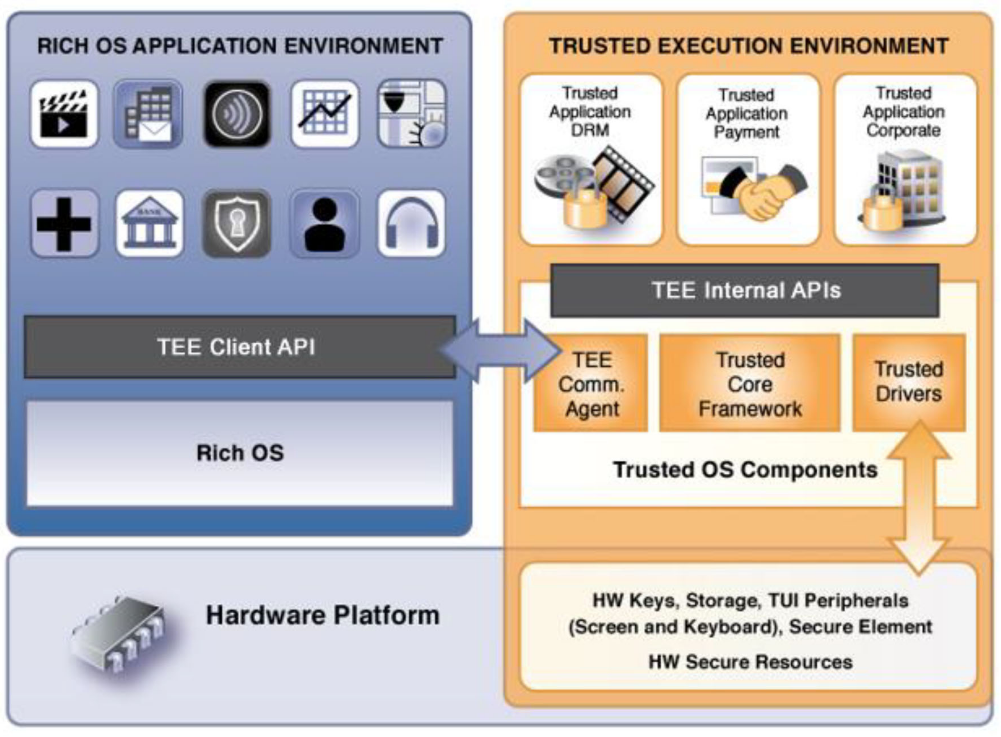
\includegraphics[width=0.5\textwidth]{img/Tee and REE.png}
  \label{fig:tee and ree}
  \caption{Trusted Execution Environment and Rich Execution
  Environment}
\end{figure}

As you can see from figure \ref{fig:tee and ree}, one one device can
run different enviroments at the same time On of those is a
\textbf{Rich Execution Environment} (REE), which is the normal
environment in which one runs any applications or OS. On the other
hand, the TEE is a separate environment isolated from the rest of the
system to run critical tasks and has access to some trusted ankles
like the hwardware keys, the secure storage, peripherals, etc.
TEE can only run on some specific hardware platform made up of trusted
components(not trustworthy, but trusted): the trusted drivers, the
core framework(the execution core) and a set of API accessible only
from trusted applications, the TEE communication agent 

In modern computing, TEE has become an important subject, especially
in the field of "confidential computing," which is actively promoted
by the Confidential Computing Consortium (CCC). The primary goal of
TEE is to protect "data in use," ensuring that nobody else can read or
write the data. Only authorized applications are allowed to process
the data. This approach contrasts with various cryptographic
techniques used to protect "data at rest" and "data in motion."

A key component of TEE, necessary to provide it's services, is the
\textbf{Root of Trust} (RoT), which is an element whose misbehavior
cannot be detected during runtime. The RoT must be \textbf{both
trusted and trustworthy}. It is also part of the Trusted Computing
Base (TCB), which is the set of hardware, firmware, and software
components critical to the system's security. Any vulnerability within
the TCB poses a significant threat to the system’s overall security.

\subsection{TEE Security Principles}

The security principles of a Trusted Execution Environment 
(TEE) involve the following:

\begin{itemize}
    \item Being part of the device's secure boot chain (based on a Root 
    of Trust) and verifying code integrity during each device boot.
    \item Hardware-based isolation from the device’s rich OS 
    environment to execute sensitive code.
    \item Isolation of Trusted Applications (TAs) from each other.
    \item Secure data storage, using a hardware-unique key accessible 
    only by the TEE OS to prevent unauthorized access, modification, 
    and any possibility of data exploitation on other devices.
    \item Privileged and secure access to peripherals (trusted path).
    \item Hardware isolation of peripherals (e.g., fingerprint sensors, 
    displays, touchpads) from the rich OS environment, controlled 
    only by the TEE during specific actions, with no visibility or 
    access by the Rich Execution Environment (REE), including 
    malware.
\end{itemize}

\section{Some TEE Implementations}
\subsection{Intel Identity Protection Technology (Intel IPT)}

Intel Identity Protection Technology (Intel IPT) is a security feature
that operates on a dual-CPU system within Intel processors. This
design leverages the Management Engine (ME), a dedicated CPU that
exists alongside the primary CPU in Intel processors. While the
primary CPU executes user tasks, the ME, integrated into the chipset,
can perform various management and security functions independently.
Typically, the ME is unused in consumer devices, but in corporate
environments, it can be activated even when the device is off via
features like wake-on-LAN, allowing remote management over Wi-Fi or
Ethernet.

Intel IPT uses the ME to run a \textbf{Java applet} isolated from the
main CPU, offering enhanced security for tasks such as cryptographic
key generation and storage, which integrates seamlessly with the
Windows Cryptographic API. Additionally, Intel IPT supports secure
One-Time Password (OTP) generation, as seen in applications like
VASCO's MYDIGIPASS.COM, which use the ME to securely store secrets for
OTPs. Another significant feature is secure PIN entry, where the
chipset manages video output to ensure the security of PIN input by
isolating it from the main system.

The ME's integration into the hardware, running on separate CPU
architecture, exemplifies a physically separated Trusted Execution
Environment (TEE), offering distinct security advantages by isolating
critical operations from the main processing tasks.

\subsection{ARM TrustZone}

ARM TrustZone is a Trusted Execution Environment (TEE) implemented in
certain ARM CPUs, designed to provide a secure and a normal mode
within the same processor. To achieve this, TrustZone extends the
CPU's bus with an additional "33rd bit" that signals whether the
processor is in secure or normal mode. This signal is exposed outside
the CPU, which enables secure peripherals and secure RAM by allowing
the system designer to control access to memory and devices based on
the security mode.

While the TrustZone framework is open and well-documented, it has some
limitations. TrustZone can only support a single secure enclave at a
time, and this security relies on software-based separation between
applications rather than on distinct hardware boundaries, making it
somewhat less secure than fully hardware-isolated environments. ARM is
actively working to expand TrustZone by introducing a third
operational mode to accommodate specific features like attestation.
However, adding this capability presents challenges due to backward
compatibility concerns, as ARM aims to preserve the success of its
platform without disrupting existing applications.

\subsection{Trustonic}

The main issue with TrustZone is that it only one secure enclave. 
To address this issue, Gemalto developed the Trusted Foundations 
system, and Giesecke+Devrient (G+D) created MobiCore. 
Both solutions effectively divide the single secure enclave into 
multiple enclaves by leveraging a smart-card operating system. 
Trustonic’s development is based on MobiCore, requiring 
license fees for implementing the code. Trustonic's TEE OS, 
named "Kinibi," includes enhancements such as version 500, 
which supports 64-bit Symmetric Multiprocessing (SMP) for 
embedded systems. Samsung Knox presents a similar approach 
but additionally incorporates secure boot functionality.

\subsection{Intel SGX}

Intel Software Guard Extensions (SGX) are closely integrated with 
the CPU and modify memory management to enhance security. 
Enclaves, which are isolated execution environments, are protected 
from other code and vice versa. As these enclaves are created, 
the code is measured in a manner akin to the Trusted Platform 
Module (TPM). SGX can also be combined with Intel Identity 
Protection Technology (IPT) to facilitate a trusted display. 
Initially, SGX1 was available on both low-end and high-end CPUs, 
while SGX2 is now primarily restricted to server-oriented CPUs, 
such as the Xeon series.

\subsection{Keystone}

Keystone is an open-source framework designed for building Trusted
Execution Environments (TEEs). It allows developers to select only the
necessary features, which helps minimize the Trusted Computing Base
(TCB), because smaller the trust "surface" the better. The
architecture consists of an untrusted environment, such as a
general-purpose operating system, combined with multiple trusted and
segregated enclaves. Keystone is built on top of RISC-V, which offers
customizable open-source hardware options, including
Field-Programmable Gate Arrays (FPGAs) or System-on-Chip (SoC)
designs. The framework incorporates core components along with
cryptographic extensions and supports various execution modes,
including Machine, Supervisor, and User modes. Additionally, it
features Physical Memory Protection (PMP) to safeguard memory and I/O
operations.

Usually, TEEs are rigid and un-customizable, with many design
implementation dictated from the underlying hardware, for example
Intel SGX has a large software stack that is not customizable, AMD SEV
have very large TCB, ARM TrustZone has a single TEE. 

The architecture is shown in figure \ref{fig:keystone}. Keystone is
structured to have a Security Monition as the only program running in
Machine mode, which provides mediation for the operations of the 
Untrusted hardware and enclaves to the Trusted hardware.
Keystone doesn't require an entire operating system to run, but only
a stripped down version because each enclave have an isolated Runtime
on top of which the Enclave app runs.

\begin{figure}[H]
  \centering
  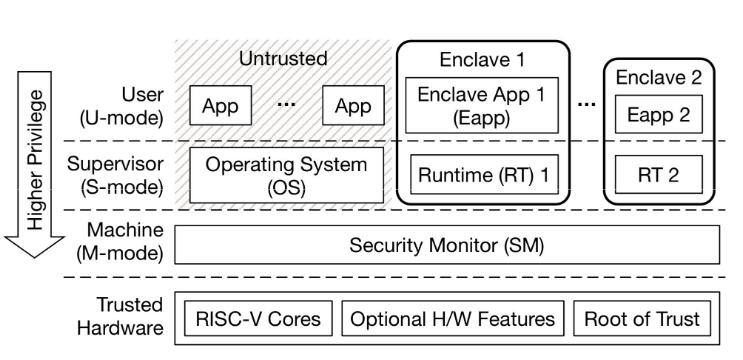
\includegraphics[width=0.6\textwidth]{img/keystone architecture.png}
  \label{fig:keystone}
  \caption{Keystone architecture}
\end{figure}

\section{Trusted computing and remote attestation}
Attacker would obviously like to inject malwares at the lowest level
possible, this is to remain undetected while still having access to
the largest part of the system. For this reason the ideal scenario is
to modify the OS is possible, or, alternatively boot an alternative
one under the control of the attacker by modifying the boot sequence
or even the bootloader.

It comes natural after this that the boot system nd the OS should be
protected: for boot sequencing we once had the BIOS, which was 
very difficult to protect, then we had UEFI, which is more secure with
native support for firmware signature and verification. After this has
been initialized, the OS can be verified before activation.

\subsection{Rootkits}
This is the generic name for a tool that allows to have root access to
a machine.

\paragraph{Firmware Rootkits} Firmware rootkits function by
overwriting the BIOS/UEFI or other hardware firmware. This allows the
rootkit to start running before the operating system even begins to
load.

\paragraph{Bootkits} Bootkits replace the bootloader of the operating
system, ensuring that the bootkit is loaded first when the node is
booted, which occurs before the OS itself initializes.

\paragraph{Kernel Rootkits} Kernel rootkits manipulate a section of
the OS kernel, enabling them to start automatically whenever the
operating system loads, embedding themselves within the core processes
of the OS.

\paragraph{Driver Rootkits} Driver rootkits disguise themselves as
trusted drivers used by the operating system (e.g., Windows) to
interact with hardware. By mimicking a legitimate driver, these
rootkits gain access to hardware resources while avoiding detection.

\section{Root of trust}
In general, protecting software withs software can not always be the
best idea, as it may fail or have bugs. For this reason, we need
hardware support to protect the software.
For this reason we have a \textbf{Root of Trust}, which is a hardware 
component that is trusted to behave as expected, and is the foundation
for the chain of trust. The RoT should be always part of the Trusted
Computing Base because hardware is anyway operated by software or
firmware
\subsection{SW root-of-trust}

An example from HPE illustrates a method of firmware 
self-protection using a software root-of-trust. HPE implements 
a designated “signature” region at a fixed location within the 
final BIOS image, which is typically 16MB in size. Keep in mind that
this was developed before UEFI.

During manufacturing, the SHA-256 hash of specific BIOS 
regions is calculated. These regions include static code, BIOS 
version information, and microcode. The computed hash is then 
sent to an HPE signing server, which returns a signed hash 
image (32 bytes) that includes the signature and certificate 
information. This signed hash image is stored in the BIOS 
“signature” region.

On power-up, the early BIOS code calculates a hash from the 
specified valid BIOS regions and verifies the validity of the 
stored “signature” contents. If the calculated hash matches 
the stored hash, the boot process proceeds; otherwise, the 
system halts, preventing further booting.

\subsection{HW root-of-trust}

A hardware root-of-trust for firmware protection typically includes 
self-verification, where a static portion of the firmware authenticates 
the updatable section. This approach allows for an internal method 
of validating firmware integrity directly within the firmware itself. 
Alternatively, firmware verification can be managed by an external 
chip, offering a secure, independent means of affirming firmware 
authenticity.

Another level of hardware root-of-trust can be implemented through 
an external cryptographic chip, which takes on the role of validating 
the BIOS in SPI flash memory after power-on. Upon successful 
validation, this chip allows the x86 CPU to exit its reset state; 
otherwise, the CPU remains in reset, ensuring security.

The external chip may also include a fusing option, allowing a public 
key hash to be securely fused and later used to verify the signature 
of the hash stored in the BIOS's signature region. This validation 
process is similar to the internal BIOS self-integrity check, with the 
added benefit of relying on an external chip, making it the true 
hardware root-of-trust.

\begin{figure}[H]
  \centering
  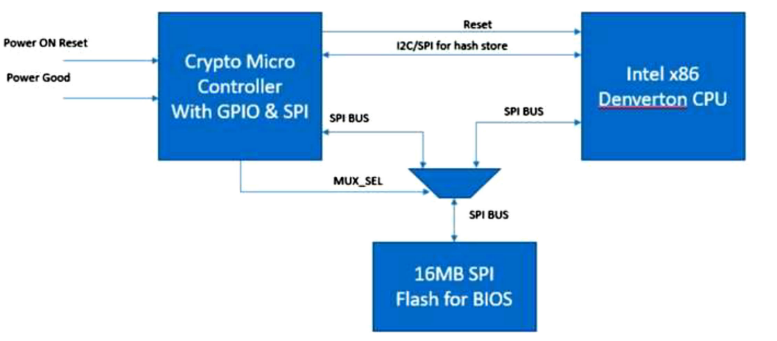
\includegraphics[width=0.6\textwidth]{img/Hw RoT verification.png}
\end{figure}
\section{Boot Types}

Different types of boot processes provide varying levels of security 
during system startup:

\paragraph{Plain Boot} A plain boot involves no security checks, 
leaving the platform vulnerable to unauthorized modifications.

\paragraph{Secure Boot} In a secure boot process, firmware verifies 
a signature before proceeding. If the verification fails, the platform 
halts, ensuring security from the earliest stages. This process is 
primarily hardware-based and verifies components up to the 
OS-loader.

\paragraph{Trusted Boot} A trusted boot involves the operating 
system verifying signatures of critical OS components, such as 
drivers and antimalware software. If any verification fails, system 
operations are halted. This type of boot is mainly software-based 
and extends verification up to the operational state of the OS.

\paragraph{Measured Boot} During a measured boot, the system 
measures each component executed from boot through a defined 
point, denoted as \(X\). Unlike other boot types, measured boot 
does not halt operations if verification fails. Instead, it can securely 
report these measurements to an external verifier, providing 
ongoing insight into system integrity.

% 2 figures 
\begin{figure}[H]
  \centering
  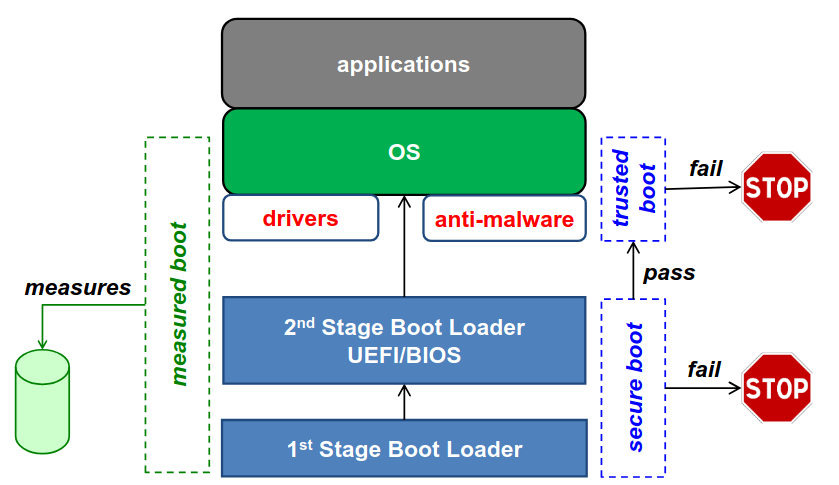
\includegraphics[width=0.6\textwidth]{img/boot types.png}
  \caption{Boot types}
\end{figure}

\section{Trusted Computing}

Trusted Computing encompasses systems and components designed 
to behave predictably and as expected. In this context, a component 
or platform is considered \textit{trusted} if it consistently performs 
according to predefined expectations, though this does not inherently 
mean it is secure or “good.” Trust in such systems requires verification 
against an expected behavior, rather than an implicit assumption of 
reliability.

A key concept within Trusted Computing is \textit{attestation}, which 
provides verifiable evidence of a platform’s state, allowing assessment 
against a known standard. Another fundamental concept is the 
\textit{Root of Trust}, an inherently trusted component within the 
system that forms the basis for verifying trustworthiness.

Trusted Computing schemes establish trust in a platform by 
identifying its hardware and software components, often through 
a \textit{Trusted Platform Module} (TPM). The TPM plays a crucial 
role in collecting and reporting component identities, offering a way 
to assess hardware and software configurations. This enables 
determination of whether a system’s behavior aligns with expected 
standards, thus supporting the establishment of trust in the platform’s 
integrity.

\subsection{Trusted Computing Base (TCB)}

The Trusted Computing Base (TCB) refers to the collection of 
system resources, including both hardware and software, that is 
fundamental in upholding the security policy of a system. An essential 
aspect of the TCB is its resilience against compromise; it must be 
able to protect itself from threats posed by any hardware or software 
outside of the TCB itself.

It is important to note that a \textit{Trusted Platform Module} (TPM) 
is not synonymous with the TCB of a system. Instead, the TPM 
serves as a tool for an independent entity to assess whether the 
TCB has been compromised. In specific implementations, the TPM 
may also play a preventative role, ensuring that the system does 
not start if the TCB fails to initialize correctly, thus providing an 
additional layer of security assurance.

\subsection{Root of Trust (RoT)}

The \textit{Root of Trust} (RoT) refers to a component within a system 
that must reliably act in an expected manner, as any deviation in its 
behavior cannot be detected. The RoT is essential in establishing trust 
within a platform and comprises several foundational components.

The \textit{Root of Trust for Measurement (RTM)} is responsible for 
taking integrity measurements and transmitting these to the 
\textit{Root of Trust for Storage} (RTS). Typically, the CPU executes 
the \textit{Core Root of Trust for Measurement} (CRTM) at boot, 
serving as the first element of BIOS/UEFI code to initiate the 
chain of trust.

The \textit{Root of Trust for Storage (RTS)} provides a shielded and 
secure storage environment for critical integrity measurements.

The \textit{Root of Trust for Reporting (RTR)} securely reports the 
content stored in the RTS, thus enabling verification of the system's 
integrity.

\subsection{Chain of Trust}

In a \textit{Chain of Trust}, each component verifies the integrity of 
the next component in sequence. Component A measures Component B and 
stores this measurement in the \textit{Root of Trust for Storage} (RTS). 
Then, Component B measures Component C and similarly stores the 
measurement in the RTS, continuing this process down the chain.

Typically, Component A is the \textit{Core Root of Trust for Measurement} 
(CRTM), which is part of the \textit{Trusted Computing Base} (TCB). By 
using the \textit{Root of Trust for Reporting} (RTR), a verifier can 
securely retrieve the measurements of Components B and C from the RTS. 
For Components B and C to be trusted, Component A must itself be 
trustworthy.

\subsection{Trusted Platform Module (TPM) Overview}

The Trusted Platform Module (TPM) is an inexpensive component,
typically costing less than 1 dollar, and is available on most servers,
laptops, and PCs. It is designed to be tamper-resistant, although it
is important to note that it is not entirely tamper-proof.

While the TPM provides security features, it is not a high-speed
cryptographic engine; in fact, it is relatively slow in terms of
processing speed. The TPM is certified with a Common Criteria
Evaluation Assurance Level (EAL) of 4 or higher, which indicates a
certain level of security assurance.

As a passive component, the TPM requires the CPU to drive its
operations. It does not have the capability to prevent the boot
process; however, it can protect sensitive data and securely report
this information. Consequently, the TPM functions as both the
\textit{Root of Trust for Storage} (RTS) and the \textit{Root of Trust
for Reporting} (RTR), but it does not serve as the \textit{Root of
Trust for Measurement} (RTM).

The TPM provides secure storage capabilities, functioning as a secure
storage component (RTS) with an extend-only approach. It can report
the content of this secure storage using a digital signature, thus
acting as a reporting entity (RTR).

One of the critical features of the TPM is its hardware random number
generator, which supports various cryptographic algorithms, including
hashing, Message Authentication Code (MAC), and both symmetric and
asymmetric encryption. However, it is important to clarify that the
TPM is not a crypto accelerator, as its performance is relatively
slow.

The TPM also facilitates the secure generation of cryptographic keys
for limited use cases. It supports binding, which encrypts data using
the TPM bind key—a unique RSA key derived from a storage key.
Additionally, the TPM allows for sealing, a process similar to
binding, but it also specifies the TPM state required for the data to
be decrypted, known as unsealed.

Furthermore, computer programs can utilize a TPM to authenticate
hardware devices. Each TPM chip is manufactured with a unique and
secret Endorsement Key (EK) that is burned in during production,
ensuring that the authenticity of the hardware can be verified.

\subsection{TPM 1.2}

TPM 1.2 features a fixed set of cryptographic algorithms, which
include SHA-1, RSA, and optionally AES. This version of the TPM
provides a single storage hierarchy specifically for the platform
user, ensuring that key management and storage are centralized.

At the core of TPM 1.2 is a single root key known as the Storage Root
Key (SRK), which is typically an RSA-2048 key. This root key serves as
the foundation for other keys within the TPM, facilitating secure
storage and cryptographic operations.

Additionally, TPM 1.2 incorporates a built-in Endorsement Key (EK)
that provides a hardware identity for the platform. This EK is
essential for establishing the authenticity of the TPM and the device
it resides in. 

Another important feature of TPM 1.2 is its capability for sealing
data to a Platform Configuration Register (PCR) value. This sealing
process ensures that the data can only be decrypted when the platform
is in a specific, verified state, enhancing the security of sensitive
information.

\subsection{TPM 1.2}

TPM 1.2 features a fixed set of cryptographic algorithms, which
include SHA-1, RSA, and optionally AES. This version of the TPM
provides a single storage hierarchy specifically for the platform
user, ensuring that key management and storage are centralized.

At the core of TPM 1.2 is a single root key known as the Storage Root
Key (SRK), which is typically an RSA-2048 key. This root key serves as
the foundation for other keys within the TPM, facilitating secure
storage and cryptographic operations.

Additionally, TPM 1.2 incorporates a built-in Endorsement Key (EK)
that provides a hardware identity for the platform. This EK is
essential for establishing the authenticity of the TPM and the device
it resides in. 

Another important feature of TPM 1.2 is its capability for sealing
data to a Platform Configuration Register (PCR) value. This sealing
process ensures that the data can only be decrypted when the platform
is in a specific, verified state, enhancing the security of sensitive
information.

\subsubsection{Implementations of TPM 2.0}

TPM 2.0 has several implementation forms, each designed to fit
different hardware and software architectures. The Discrete TPM is a
dedicated chip that implements TPM functionality within its own
tamper-resistant semiconductor package, providing robust security.

In contrast, the Integrated TPM is part of another chip and is not
required to implement tamper resistance. For example, Intel has
integrated TPMs in some of its chipsets, balancing functionality with
space and cost considerations.

The Firmware TPM is a software-only solution that operates within a
CPU's trusted execution environment. Major manufacturers such as AMD,
Intel, and Qualcomm have implemented firmware TPMs, allowing for
flexibility in system design.

Another form is the Hypervisor TPM, which offers a virtual TPM managed
by a hypervisor. This runs in an isolated execution environment and is
comparable to a firmware TPM in terms of security and functionality.

Finally, the Software TPM serves as a software emulator of a TPM,
primarily useful for development purposes. This allows developers to
test and implement TPM functionalities without needing dedicated
hardware.

\subsubsection{TPM 2.0 Three Hierarchies}

TPM 2.0 defines three key hierarchies, each serving distinct purposes
and managing different aspects of security and key storage.

The first hierarchy is the Platform Hierarchy, which is dedicated to
managing the platform’s firmware. This hierarchy utilizes non-volatile
(NV) storage for keys and data, ensuring that critical
firmware-related information is securely maintained.

The second is the Endorsement Hierarchy, which primarily caters to the
privacy administrator. Similar to the Platform Hierarchy, this one
also provides storage for keys and data, emphasizing the importance of
privacy in the overall security architecture.

Lastly, the Storage Hierarchy is designed for the platform’s owner,
who typically also acts as the privacy administrator. This hierarchy
features NV storage for keys and data, allowing for efficient
management of cryptographic assets.

Each of these hierarchies comes with dedicated authorization
mechanisms, such as passwords, and specific policies to govern access
and usage. Additionally, each hierarchy utilizes a unique seed for
generating the primary keys, further enhancing the security and
integrity of the TPM's operations.

\subsection{Using a TPM for Securely Storing Data}

Utilizing a Trusted Platform Module (TPM) for securely storing data
involves several key considerations to ensure both security and
accessibility.

One primary advantage of using a TPM is its physical isolation. The
storage occurs within the TPM itself, specifically in non-volatile RAM
(NVRAM), which helps safeguard sensitive information. This storage can
include primary keys and permanent keys, although it is important to
note that the space available in a TPM is very limited.

To enhance security, Mandatory Access Control (MAC) mechanisms are
employed, which govern how data and keys are accessed within the TPM.
This cryptographic isolation ensures that even if data is stored
outside the TPM, such as on a platform's hard drive or solid-state
drive (SSD), it remains protected.

When storing keys or data outside the TPM, it is crucial that the
information is encapsulated in a secure format, often referred to as a
blob. This blob must be protected, typically by encrypting it with a
key controlled by the TPM. The use of MAC further reinforces the
security measures, ensuring that access to the stored data is tightly
regulated.

\subsection{TPM Objects}

Trusted Platform Modules (TPMs) utilize various objects to manage
cryptographic keys and secure data. One of the primary types of
objects within a TPM is the primary key, which includes endorsement
keys and storage keys. These keys are derived from one of the primary
seeds stored within the TPM. Notably, the TPM does not return the
private value of these keys; instead, they can be re-created using the
same parameters, assuming that the primary seed remains unchanged.

In addition to primary keys, TPMs also handle keys and sealed data
objects (SDOs). These objects are protected by a Storage Parent Key
(SPK), which is necessary within the TPM to load or create a key or
SDO. The randomness required for key generation and other
cryptographic functions is provided by the TPM's built-in Random
Number Generator (RNG). 

When a key is generated, the TPM returns the private part, which is
protected by the SPK. However, it is essential to note that this
private part must be stored securely, as its integrity is critical to
maintaining the overall security provided by the TPM.

\subsection{TPM Object Areas}

Trusted Platform Modules (TPMs) categorize the storage structure of objects into distinct areas, each serving a specific purpose:

\begin{itemize}
  \item \textbf{Public Area:} This area is utilized to uniquely
    identify an object, providing essential information for the
    management of keys and data.

  \item \textbf{Private Area:} Containing the object's secrets, this
    area exists solely within the TPM. It is crucial for maintaining
    the confidentiality and integrity of the keys and data stored
    within the module.

  \item \textbf{Sensitive Area:} This consists of the encrypted
    private area, specifically designed for use when storing sensitive
    data outside of the TPM. It ensures that even when data is not
    housed within the TPM, it remains secure through encryption.
\end{itemize}

\subsection{TPM Platform Configuration Register (PCR)}

The Platform Configuration Register (PCR) serves as the Trusted
Platform Module's (TPM) implementation of Root of Trust for Storage
(RTS) and is a core mechanism for recording platform integrity. PCRs
maintain their values and can only be reset during a platform reset or
through a hardware signal, which ensures that any malicious code
cannot manipulate or retract its measurements.

PCRs are extended using a cumulative hash, following the formula:

\[
\text{PCR}_{\text{new}} = \text{hash}(\text{PCR}_{\text{old}} \, || \, \text{digest\_of\_new\_data})
\]

This process is commonly referred to as the EXTEND operation.
Additionally, PCRs can be utilized to gate access to other TPM
objects. For example, BitLocker uses PCR values to seal disk
encryption keys, ensuring that the keys can only be accessed when the
platform is in a known and trusted state.

\subsection{Measured Boot}
\begin{figure}[H]
  \centering
  \includegraphics[width=0.6\textwidth]{img/Measured boot.png}
  \caption{Measured boot}
\end{figure}
\subsection{Remote attestation procedure}
\begin{figure}[H]
  \centering
  \includegraphics[width=0.6\textwidth]{img/remote attestation
  procedure.png}
  \caption{Remote attestation procedure}
\end{figure}

\subsection{Management of Remote Attestation}

When managing remote attestation, several factors must be considered
to ensure its effectiveness. One critical aspect is whether to
implement only boot attestation, which is static, or to include
periodic (dynamic) attestation as well. This decision should take into
account the attack model, especially with respect to runtime
vulnerabilities that could be exploited.

The periodicity of the attestation operation is another important
consideration, as it must align with the speed of potential attacks.
Current implementation limits, which include the time required for
signature verification, protocol execution, and database lookups, are
typically in the range of several seconds due to the inherent slowness
of Trusted Platform Modules (TPMs).

Another challenge in remote attestation management is whitelist
generation. This process can be complex in general but may be less
difficult in limited environments, such as Internet of Things (IoT)
devices, edge devices, Software-Defined Networking (SDN), and Network
Function Virtualization (NFV). 

Furthermore, it is essential to label components appropriately—such as
good, old, buggy, or vulnerable—and to include configurations from
sources like Management and Orchestration (MANO) or network management
tools. While generating labels can be straightforward if the data is
file-based, it becomes significantly more challenging when dealing
with memory-based data.

